\documentclass{ximera}

\usepackage{epsfig}

\graphicspath{
  {./}
  {figures/}
}


\usepackage{morewrites}

%\newcounter{ccounter}
%\setcounter{ccounter}{1}
%\newcommand{\Chapter}[1]{\setcounter{chapter}{\arabic{ccounter}}\chapter{#1}\addtocounter{ccounter}{1}}

%\newcommand{\section}[1]{\section{#1}\setcounter{thm}{0}\setcounter{equation}{0}}

%\renewcommand{\theequation}{\arabic{chapter}.\arabic{section}.\arabic{equation}}
%\renewcommand{\thefigure}{\arabic{chapter}.\arabic{figure}}
%\renewcommand{\thetable}{\arabic{chapter}.\arabic{table}}

%\newcommand{\Sec}[2]{\section{#1}\markright{\arabic{ccounter}.\arabic{section}.#2}\setcounter{equation}{0}\setcounter{thm}{0}\setcounter{figure}{0}}

\newcommand{\Sec}[2]{\section{#1}}

\setcounter{secnumdepth}{2}
%\setcounter{secnumdepth}{1} 

%\newcounter{THM}
%\renewcommand{\theTHM}{\arabic{chapter}.\arabic{section}}

\newcommand{\trademark}{{R\!\!\!\!\!\bigcirc}}
%\newtheorem{exercise}{}

\newcommand{\dfield}{{\sf dfield9}}
\newcommand{\pplane}{{\sf pplane9}}

\newcommand{\EXER}{\section*{Exercises}}%\vspace*{0.2in}\hrule\small\setcounter{exercise}{0}}
\newcommand{\CEXER}{}%\vspace{0.08in}\begin{center}Computer Exercises\end{center}}
\newcommand{\TEXER}{} %\vspace{0.08in}\begin{center}Hand Exercises\end{center}}
\newcommand{\AEXER}{} %\vspace{0.08in}\begin{center}Hand Exercises\end{center}}

% BADBAD: \newcommand{\Bbb}{\bf}

\newcommand{\R}{\mbox{$\Bbb{R}$}}
\newcommand{\C}{\mbox{$\Bbb{C}$}}
\newcommand{\Z}{\mbox{$\Bbb{Z}$}}
\newcommand{\N}{\mbox{$\Bbb{N}$}}
\newcommand{\D}{\mbox{{\bf D}}}
\usepackage{amssymb}
%\newcommand{\qed}{\hfill\mbox{\raggedright$\square$} \vspace{1ex}}
%\newcommand{\proof}{\noindent {\bf Proof:} \hspace{0.1in}}

\newcommand{\setmin}{\;\mbox{--}\;}
\newcommand{\Matlab}{{M\small{AT\-LAB}} }
\newcommand{\Matlabp}{{M\small{AT\-LAB}}}
\newcommand{\computer}{\Matlab Instructions}
\newcommand{\half}{\mbox{$\frac{1}{2}$}}
\newcommand{\compose}{\raisebox{.15ex}{\mbox{{\scriptsize$\circ$}}}}
\newcommand{\AND}{\quad\mbox{and}\quad}
\newcommand{\vect}[2]{\left(\begin{array}{c} #1_1 \\ \vdots \\
 #1_{#2}\end{array}\right)}
\newcommand{\mattwo}[4]{\left(\begin{array}{rr} #1 & #2\\ #3
&#4\end{array}\right)}
\newcommand{\mattwoc}[4]{\left(\begin{array}{cc} #1 & #2\\ #3
&#4\end{array}\right)}
\newcommand{\vectwo}[2]{\left(\begin{array}{r} #1 \\ #2\end{array}\right)}
\newcommand{\vectwoc}[2]{\left(\begin{array}{c} #1 \\ #2\end{array}\right)}



\newcommand{\inv}{^{-1}}
\newcommand{\CC}{{\cal C}}
\newcommand{\CCone}{\CC^1}
\newcommand{\Span}{{\rm span}}
\newcommand{\rank}{{\rm rank}}
\newcommand{\trace}{{\rm tr}}
\newcommand{\RE}{{\rm Re}}
\newcommand{\IM}{{\rm Im}}
\newcommand{\nulls}{{\rm null\;space}}

\newcommand{\dps}{\displaystyle}
\newcommand{\arraystart}{\renewcommand{\arraystretch}{1.8}}
\newcommand{\arrayfinish}{\renewcommand{\arraystretch}{1.2}}
\newcommand{\Start}[1]{\vspace{0.08in}\noindent {\bf Section~\ref{#1}}}
\newcommand{\exer}[1]{\noindent {\bf \ref{#1}}}
\newcommand{\ans}{}
\newcommand{\matthree}[9]{\left(\begin{array}{rrr} #1 & #2 & #3 \\ #4 & #5 & #6
\\ #7 & #8 & #9\end{array}\right)}
\newcommand{\cvectwo}[2]{\left(\begin{array}{c} #1 \\ #2\end{array}\right)}
\newcommand{\cmatthree}[9]{\left(\begin{array}{ccc} #1 & #2 & #3 \\ #4 & #5 &
#6 \\ #7 & #8 & #9\end{array}\right)}
\newcommand{\vecthree}[3]{\left(\begin{array}{r} #1 \\ #2 \\
#3\end{array}\right)}
\newcommand{\cvecthree}[3]{\left(\begin{array}{c} #1 \\ #2 \\
#3\end{array}\right)}
\newcommand{\cmattwo}[4]{\left(\begin{array}{cc} #1 & #2\\ #3
&#4\end{array}\right)}

\newcommand{\Matrix}[1]{\ensuremath{\left(\begin{array}{rrrrrrrrrrrrrrrrrr} #1 \end{array}\right)}}

\newcommand{\Matrixc}[1]{\ensuremath{\left(\begin{array}{cccccccccccc} #1 \end{array}\right)}}



\renewcommand{\labelenumi}{\theenumi)}
\newenvironment{enumeratea}%
{\begingroup
 \renewcommand{\theenumi}{\alph{enumi}}
 \renewcommand{\labelenumi}{(\theenumi)}
 \begin{enumerate}}
 {\end{enumerate}\endgroup}



\newcounter{help}
\renewcommand{\thehelp}{\thesection.\arabic{equation}}

%\newenvironment{equation*}%
%{\renewcommand\endequation{\eqno (\theequation)* $$}%
%   \begin{equation}}%
%   {\end{equation}\renewcommand\endequation{\eqno \@eqnnum
%$$\global\@ignoretrue}}

%\input{psfig.tex}

\author{Martin Golubitsky and Michael Dellnitz}

%\newenvironment{matlabEquation}%
%{\renewcommand\endequation{\eqno (\theequation*) $$}%
%   \begin{equation}}%
%   {\end{equation}\renewcommand\endequation{\eqno \@eqnnum
% $$\global\@ignoretrue}}

\newcommand{\soln}{\textbf{Solution:} }
\newcommand{\exercap}[1]{\centerline{Figure~\ref{#1}}}
\newcommand{\exercaptwo}[1]{\centerline{Figure~\ref{#1}a\hspace{2.1in}
Figure~\ref{#1}b}}
\newcommand{\exercapthree}[1]{\centerline{Figure~\ref{#1}a\hspace{1.2in}
Figure~\ref{#1}b\hspace{1.2in}Figure~\ref{#1}c}}
\newcommand{\para}{\hspace{0.4in}}

\renewenvironment{solution}{\suppress}{\endsuppress}

\ifxake
\newenvironment{matlabEquation}{\begin{equation}}{\end{equation}}
\else
\newenvironment{matlabEquation}%
{\let\oldtheequation\theequation\renewcommand{\theequation}{\oldtheequation*}\begin{equation}}%
  {\end{equation}\let\theequation\oldtheequation}
\fi

\makeatother


\title{Coupled Linear Systems}

\begin{document}
\begin{abstract}
\end{abstract}
\maketitle

 \index{coupled system} \label{s:3.5}


The general linear constant coefficient system in two unknown functions 
$x_1,x_2$ is:
\renewcommand{\arraystretch}{1.8}c6.3.1
\begin{equation}\label{lin3}
\begin{array}{ccc}
\dps \frac{dx_1}{dt}(t) & = & ax_1(t) + bx_2(t) \\
\dps \frac{dx_2}{dt}(t) & = & cx_1(t) + dx_2(t).
\end{array}
\end{equation}
\renewcommand{\arraystretch}{1.0}%
The uncoupled systems studied in Section~\ref{sec:UncoupledLS} are obtained 
by setting $b=c=0$ in \eqref{lin3}.  We have discussed how to solve \eqref{lin3} 
by formula \eqref{e:explicitsoln} when the system is uncoupled.  We have also 
discussed how to visualize the phase plane for different choices of the 
diagonal entries $a$ and $d$.  At present, we cannot
solve \eqref{lin3} by formula when the coefficient matrix is not diagonal.
But we may use {\pplane} to solve the initial value problems numerically 
for these coupled systems.  We illustrate this point by solving
\begin{eqnarray*}
\frac{dx_1}{dt}(t) & = &  -x_1(t) + 3x_2(t) \\
\frac{dx_2}{dt}(t) & = &  3x_1(t) - x_2(t).
\end{eqnarray*}
After starting {\pplane}, select {\sf linear system} from the
{\sf Gallery} and set the constants to:
\[
	a = -1,\quad b = 3,\quad c = 3, \quad d = -1.
\]
Click on {\sf Proceed}.  In order to have equally spaced coordinates on
the $x$ and $y$ axes, do the following.   In the {\sf PPLANE8 Display} 
window click on the {\sf edit} button and then on the {\sf zoom in square} 
command.  Then, using the mouse, click on the origin.

\subsection*{Eigendirections}

After computing several solutions, we find that for increasing
time $t$ all the solutions seem to approach the diagonal line
given by the equation $x_1=x_2$. Similarly, in backward time $t$
the solutions approach the anti-diagonal $x_1=-x_2$.  In other
words, as for the case of uncoupled systems, we find two
distinguished directions in the $(x,y)$-plane.  See
Figure~\ref{F:invariantlines}.  Moreover, the computations
indicate that these lines are invariant in the sense that
solutions starting on these lines remain on them for all time.
This statement can be verified numerically by using the {\sf
Keyboard input} in the {\sf PPLANE8 Options} to choose initial
conditions $(x_0,y_0)=(1,1)$ and $(x_0,y_0)=(1,-1)$.

\begin{figure}[htb]
     \centerline{%
     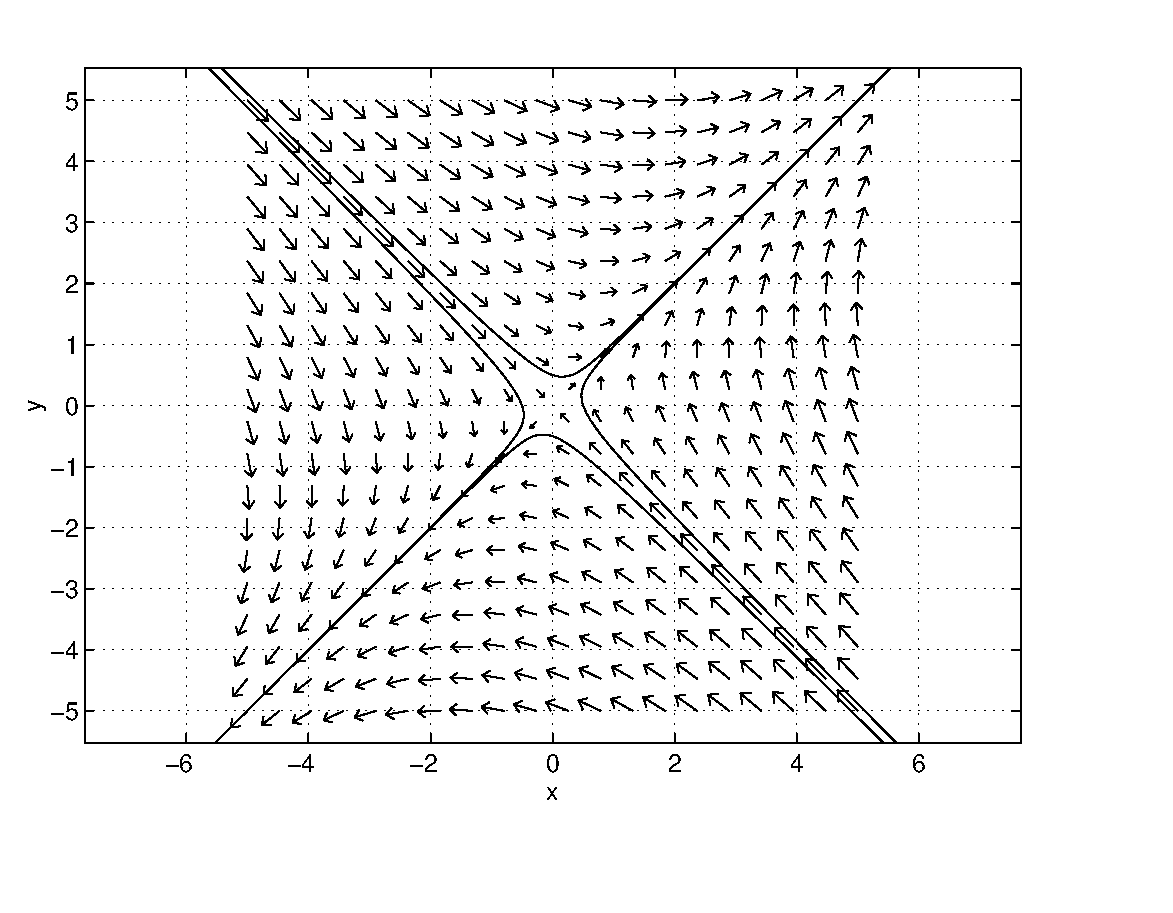
\psfig{file=../figures/invline.eps,width=3.5in}}
     \caption{{\sf PPLANE8 Display} for \protect\eqref{lin3} with
             $a=-1=d$; $b=3=c$; and $x,y\in [-5,5]$.
	Solutions going through $(\pm 0.5,0)$ and $(0,\pm 0.5)$ are shown.}
     \label{F:invariantlines}
\end{figure}

\begin{definition} \label{D:eigendirection}
An invariant line for a linear system of differential equations
is called an {\em eigendirection}\index{eigendirection}.
\end{definition}

Observe that eigendirections vary if we change parameters.  For
example, if we set $b$ to $1$, then there are still two
distinguished lines but these lines are no longer perpendicular.

For uncoupled systems, we have shown analytically that the $x$
and $y$ axes are eigendirections.  The numerical computations
that we have just performed indicate that eigendirections exist
for many coupled systems.  This discussion leads naturally to
two questions:
\begin{enumerate}
\item Do eigendirections always exist?
\item How can we find eigendirections?
\end{enumerate}
The second question will be answered in Sections~\ref{S:IVP&E} and 
\ref{S:evchp}.  We can answer the first question by performing another 
numerical computation.  In the setup window, change the parameter $b$ 
to $-2$.  Then numerically compute some solutions to see that there
are no eigendirections in the phase space of this system.  Observe that
all solutions appear to spiral into the origin as time goes to
infinity.  The phase portrait is shown in Figure~\ref{pp_dsp2}.
\begin{figure}[htb]
      \centerline{%
      \psfig{file=../figures/pp_dsp2.eps,width=3.5in}}
      \caption{{\sf PPLANE8 Display} for the {\sf linear system}
		with $a=-1$, $b=-2$, $c=3$, $d=-1$.}
      \label{pp_dsp2}
\end{figure}

\subsubsection*{Second Order Differential Equations}
\index{differential equation!second order}

We now show analytically that certain linear systems of
differential equations have no invariant lines in their phase portrait.

We do this by showing that second order differential equations can be
reduced to first order systems by a simple but important trick.  Indeed,
sometimes it is easier to solve a single second order equation, and
sometimes it is easier to solve the first order system.  At this stage
we introduce this connection by considering the differential equation
\begin{equation}  \label{E:2ndordera}
\frac{d^2x}{dt^2} + x = 0.
\end{equation}
This differential equation states that we are looking for a function
$x(t)$ whose second derivative is $-x(t)$.  From calculus, we know
that $x(t)=\cos t$ is such a function.

Let $y(t)=\dot{x}(t)$.  Then
\eqref{E:2ndordera} may be rewritten as a first order coupled system
in $x(t)$ and $y(t)$ as follows:
\begin{equation}  \label{E:2nd->1st}
\begin{array}{rcl}
\dot{x} & = & y \\
\dot{y} & = & -x.
\end{array}
\end{equation}
Observe that if $x(t)$ is a solution to \eqref{E:2ndordera}, then
\[
0 = \frac{d^2x}{dt^2} + x = \frac{dy}{dt} + x.
\]
Hence,
\[
\dot{y} = -x
\]
Conversely, if $(x(t),y(t))$ is a solution to \eqref{E:2nd->1st}, then
$x(t)$ is a solution to \eqref{E:2ndordera}.  That is,
\[
\frac{d^2x}{dt^2} + x = \frac{dy}{dt} + x = -x + x = 0.
\]

It follows from the discussion that $(x(t),y(t))=(\cos t,\sin t)$ is 
a solution to the differential equation \eqref{E:2nd->1st}.  We have shown 
analytically that the unit circle centered at the origin is a solution 
trajectory for \eqref{E:2nd->1st}.  Hence \eqref{E:2nd->1st} has no 
eigendirections.  It may be checked using \Matlab that all solution 
trajectories for \eqref{E:2nd->1st} are just circles centered at the origin.


\EXER

\CEXER

\begin{exercise} \label{c3.5.a01}
Choose the {\sf linear system} in {\pplane} and set $a=0$, $b=1$, and 
$c=-1$.  Then find values $d$ such that except for the origin itself all 
solutions appear to
\begin{itemize}
\item[(a)] spiral into the origin;
\item[(b)] spiral away from the origin;
\item[(c)] form circles around the origin;
\end{itemize}

\begin{solution}

\soln
\begin{enumeratea}
\item All trajectories converge on the origin when $D < 0$, as shown in
Figure~\ref{c3.5.a01}a, which graphs the system with $D =- 1$;

\item All trajectories move away from the origin when $D > 0$, as shown in
Figure~\ref{c3.5.a01}b, which graphs the system with $D = 1$

\item Trajectories form circles around the origin when $D = 0$, as shown in
Figure~\ref{c3.5.a01}c.
\begin{figure}[htb]
                       \centerline{%
                       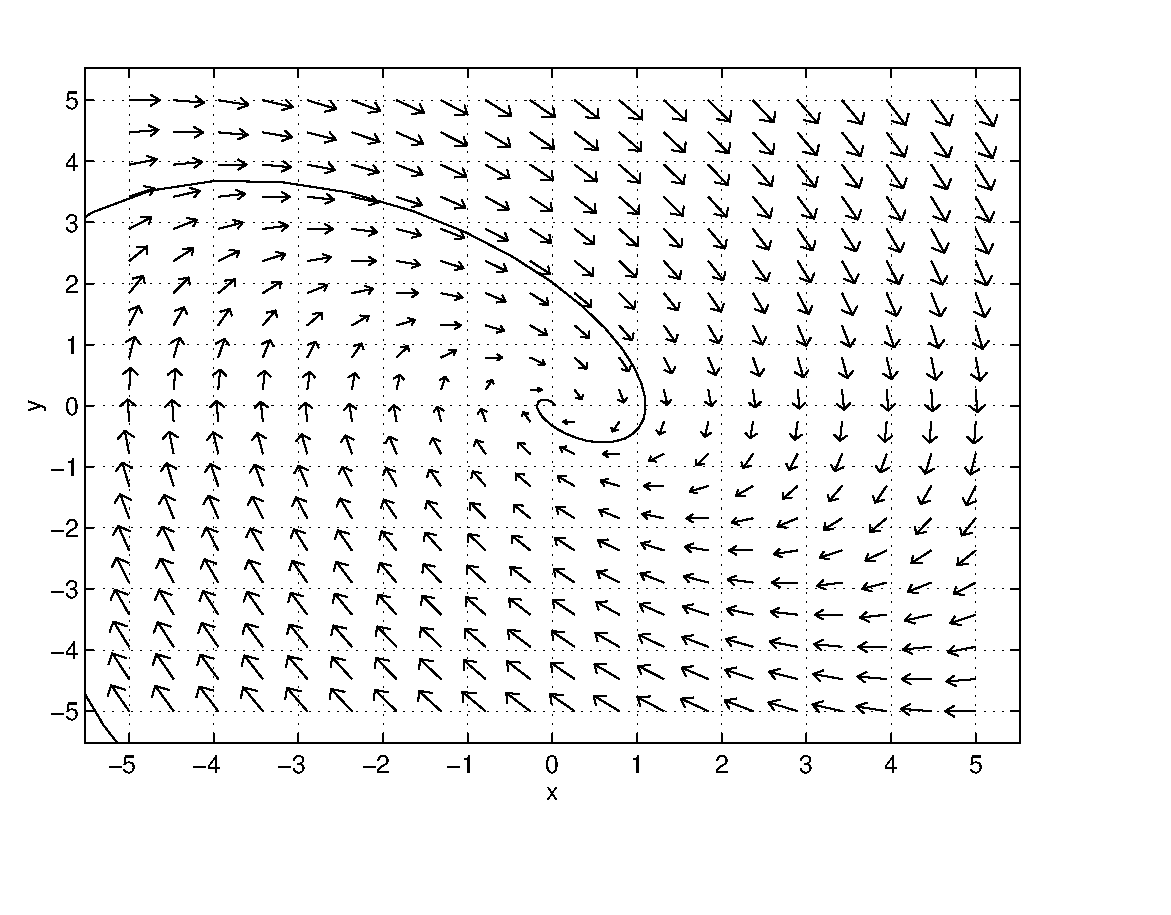
\psfig{file=exfigure/3-5-a01a.eps,width=1.8in}
                       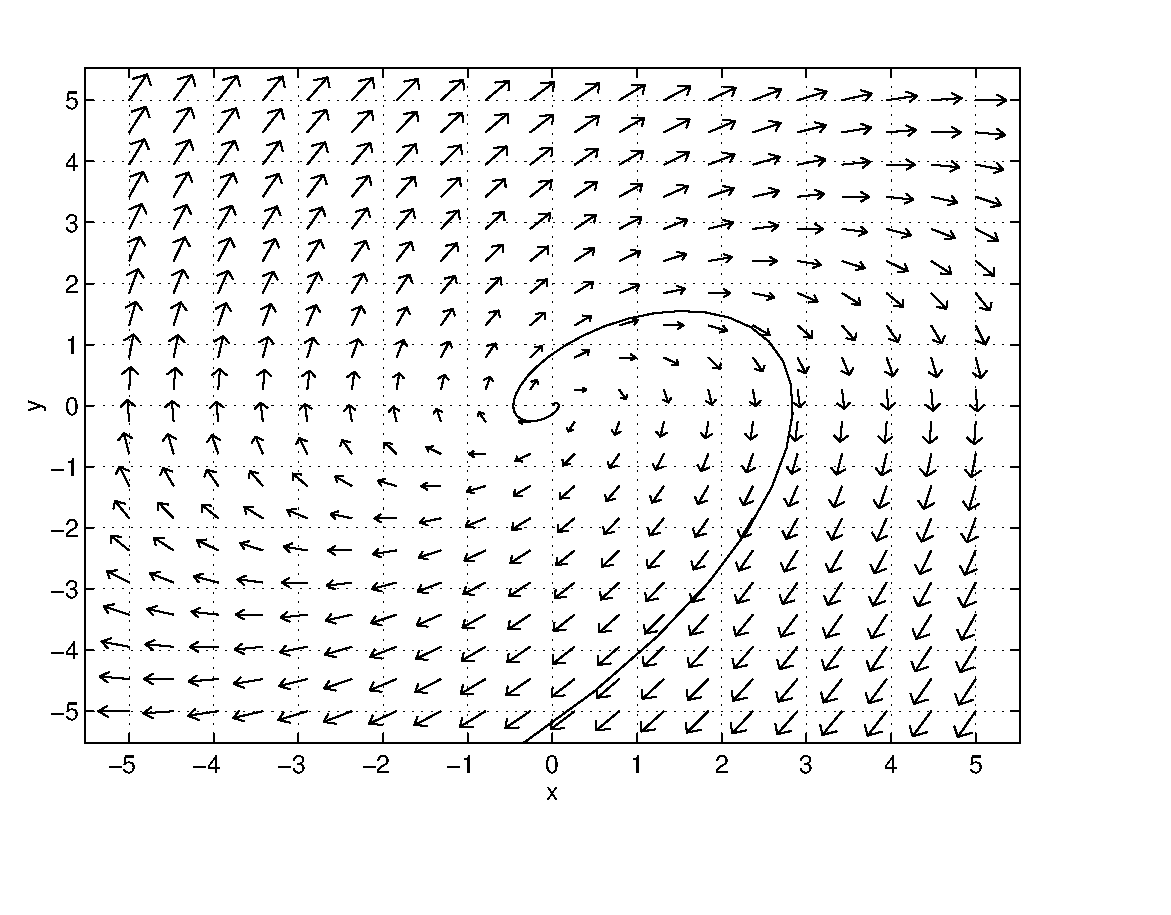
\psfig{file=exfigure/3-5-a01b.eps,width=1.8in}
                       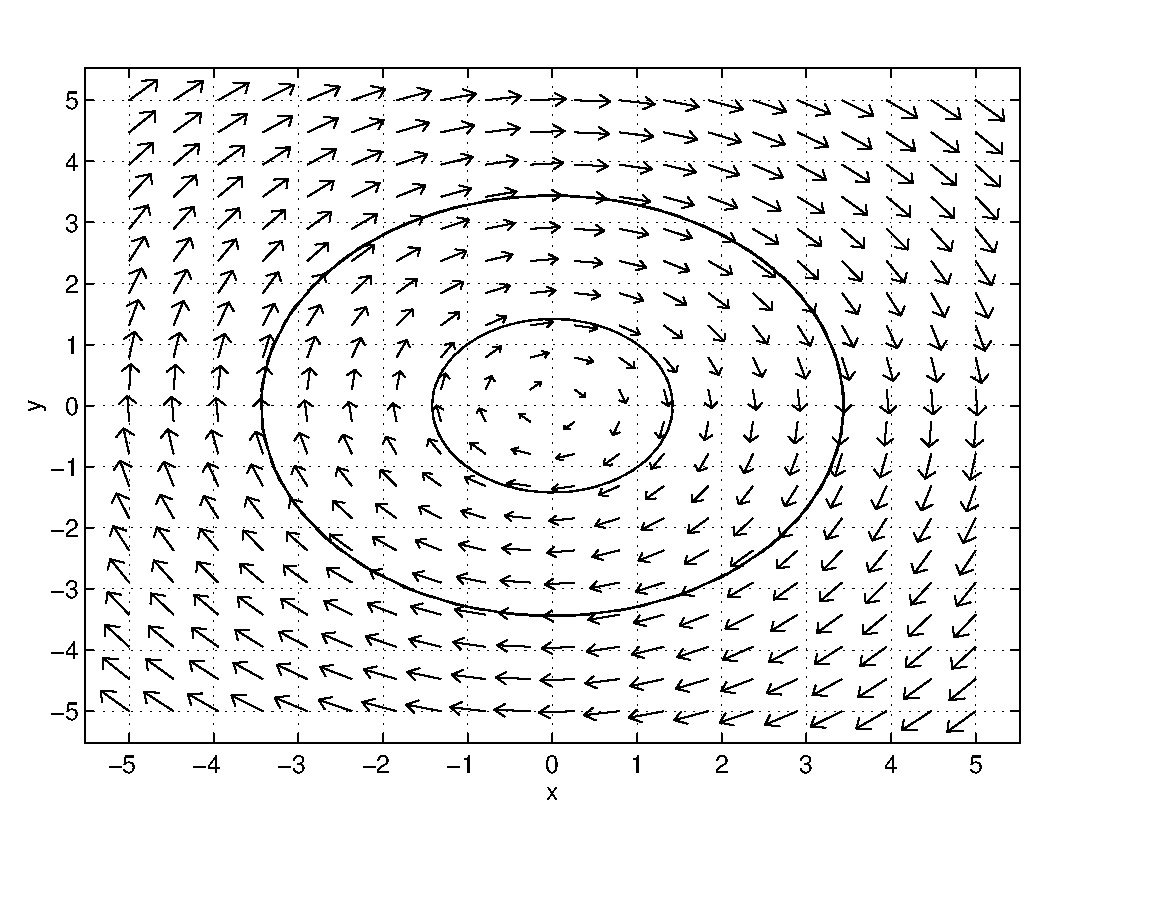
\psfig{file=exfigure/3-5-a01c.eps,width=1.8in}}
	\centerline{$D = -1$\hspace{1.4in}$D = 1$\hspace{1.4in}$D = 0$}
	\exercapthree{c3.5.a01}
\end{figure}
\end{enumeratea}
\end{solution}
\end{exercise}

\begin{exercise} \label{c3.5.2}
Choose the {\sf linear system} in {\pplane} and set
$a=-1$, $c=3$, and $d=-1$.
Then find a value for $b$ such that the behavior of the
solutions of the system is ``qualitatively'' the same as for a
diagonal system where $a$ and $d$ are negative.  In particular,
the origin should be an asymptotically stable equilibrium and
the solutions should approach that equilibrium along a
distinguished line.

\begin{solution}

\ans The solutions are similar to those for a diagonal system when
$B = 0$.

\soln At this value of $B$, the origin is a stable equilibrium, and the
solutions approach the origin tangent to the line $x = 0$.  When $B < 0$,
the graph is a spiral, so the solutions do not approach the origin along
a distinguished line.  When $B > 0$, the origin is a saddle rather
than a sink; that is, the origin is not an asymptotically stable
equilibrium.  Figure \ref{c3.5.2} shows five sample trajectories
for the system, two of which begin on the $y$-axis.

\begin{figure}[htb]
                       \centerline{%
                       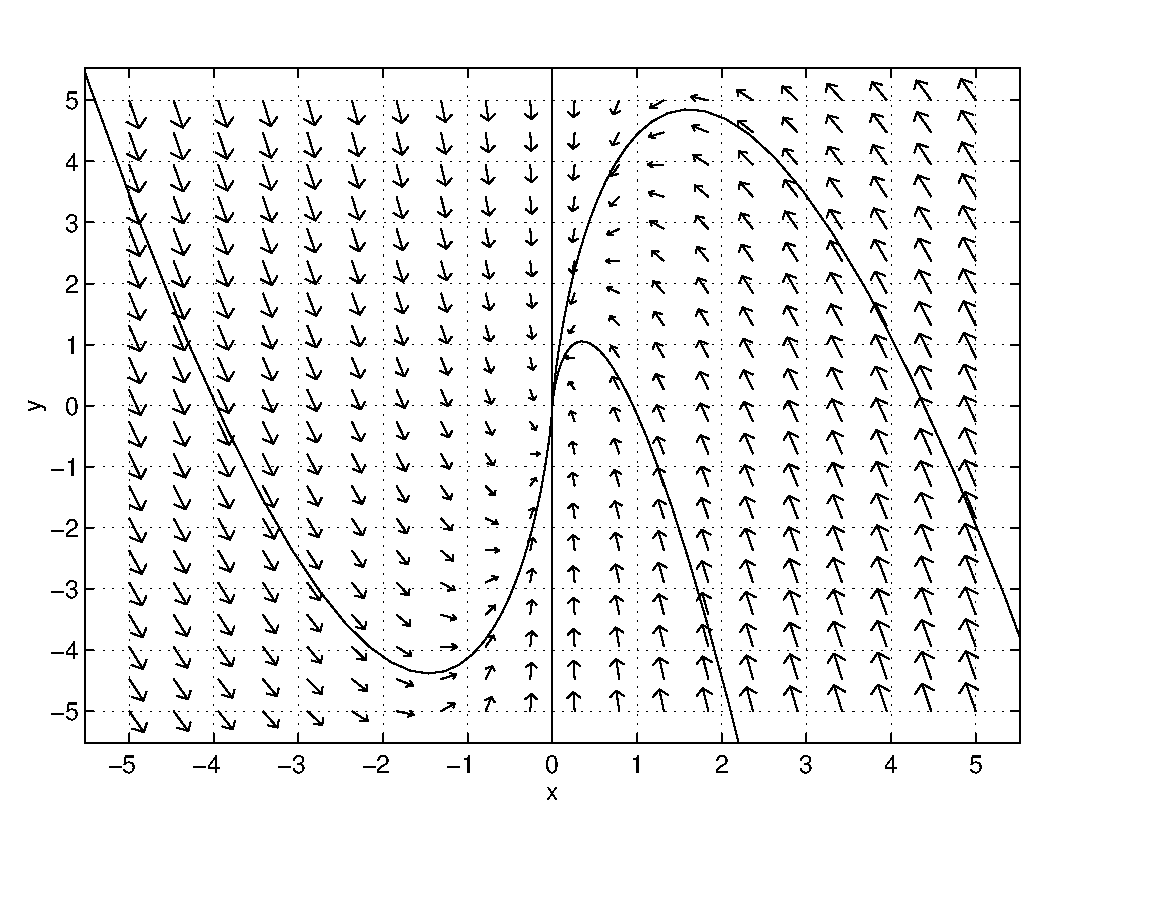
\psfig{file=exfigure/3-5-2.eps,width=3.0in}}
			\exercap{c3.5.2}	
\end{figure}

\end{solution}
\end{exercise}

\begin{exercise} \label{c3.5.3}
Choose the {\sf linear system} in {\pplane} and set
$a=d$ and $b=c$.  Verify that for these systems of differential
equations:
\begin{itemize}
\item[(a)]  When $|a|<b$ typical trajectories approach the line
$y=x$ as $t\to\infty$ and the line $y=-x$ as $t\to -\infty$.
\item[(b)]  Assume that $b$ is positive, $a$ is negative, and $b<-a$. 
With these assumptions show that the origin is a sink and that typical 
trajectories approach the origin tangent to the line $y=x$.
\end{itemize}

\begin{solution}

Graphs made in {\tt pplane5} using the {\tt axis('equal')} command
verify these statements regarding linear systems where $A = D$
and $B = C$.  Figure \ref{c3.5.3}a, uses $A = D = -1$ and
$B = C = 2$, and shows four sample trajectories which approach
the line $y = x$ as $t \rightarrow \infty$.  Figure
\ref{c3.5.3}b graphs the linear system with $A = D = -3$
and $B = C = 2$.  It shows four sample trajectories, three of
which approach the origin tangent to $y = x$.  The fourth
trajectory has an initial point $0 < x_0 = -y_0$ and approaches
the origin on the straight line $y = -x$, which is orthogonal
to $y = x$.
\begin{figure}[htb]
                       \centerline{%
                       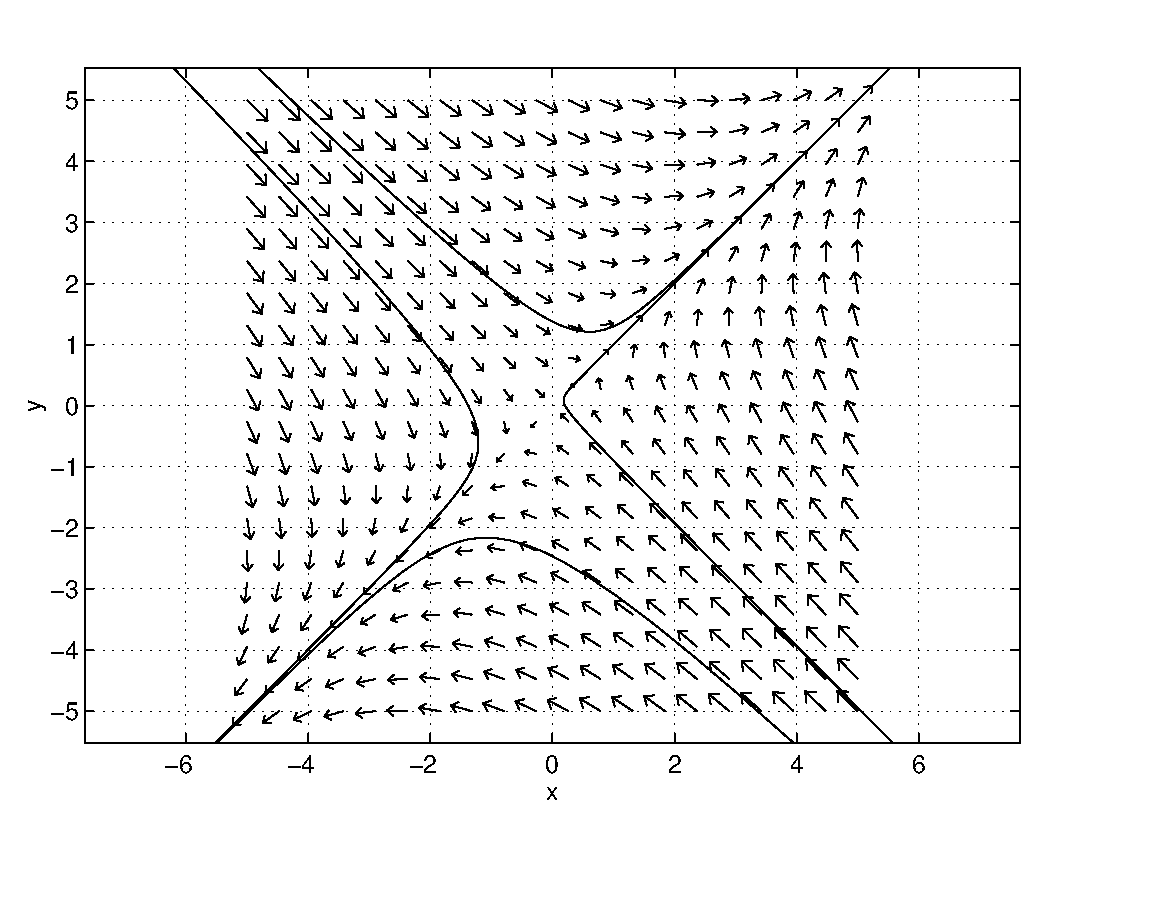
\psfig{file=exfigure/3-5-3a.eps,width=2.75in}
                       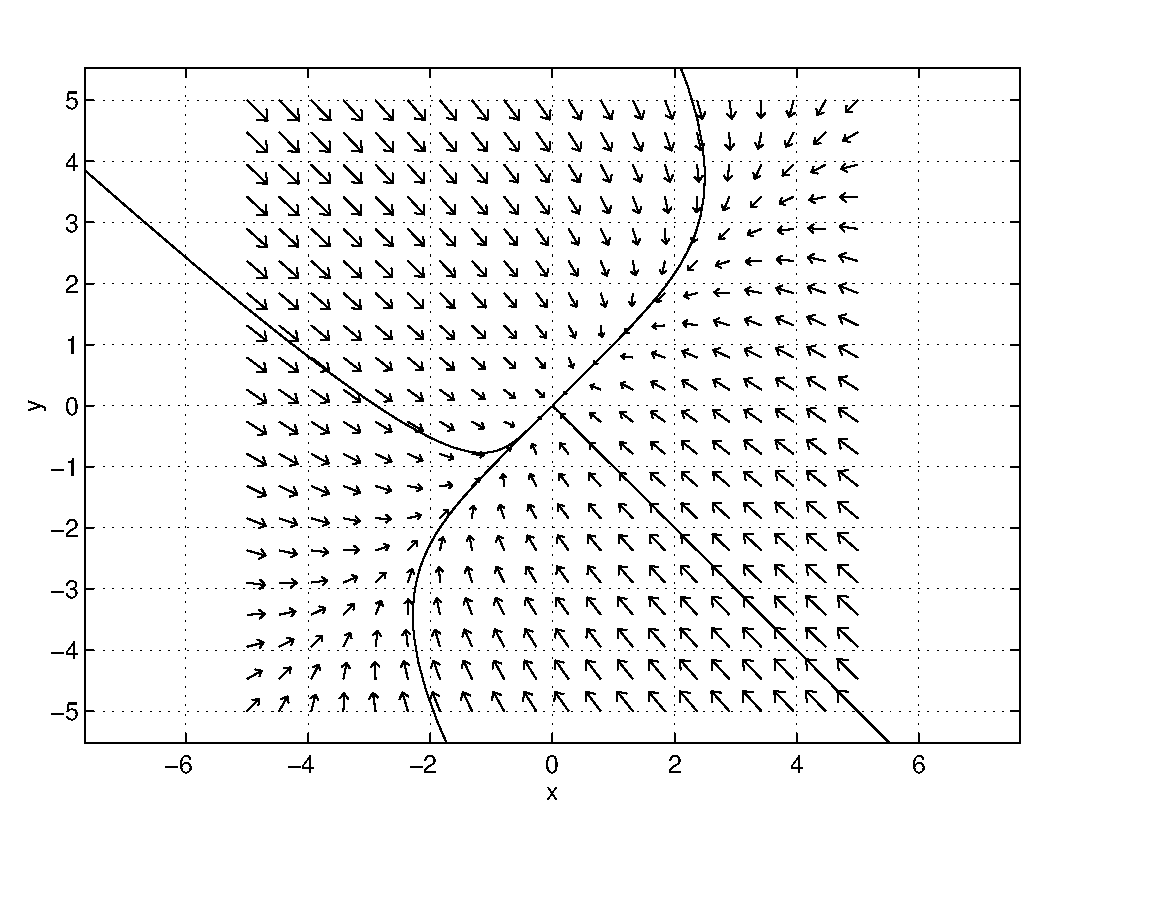
\psfig{file=exfigure/3-5-3b.eps,width=2.75in}}
			\exercaptwo{c3.5.3}	
\end{figure}

\end{solution}
\end{exercise}

\TEXER

\begin{exercise} \label{c3.5.4}
Sketch the time series $y(t)$ for the solution to the
differential equation whose phase plane is pictured in
Figure~\ref{pp_dsp2} with initial condition
$(x(0),y(0))=(\frac{1}{2},\frac{1}{2})$ .  Check your answer
using {\pplane}.

\begin{solution}

The {\tt pplane5} graph for the linear system (Figure \ref{pp_dsp2}) is
a spiral.  So as $t \rightarrow \infty$, $y$ approaches $0$ oscillating
between positive and negative values.  The graph of {\tt y vs.\ t} for the
trajectory with initial condition $(x_0,y_0) = \left(\frac{1}{2},
\frac{1}{2}\right)$ is shown in Figure \ref{c3.5.4}.

\begin{figure}[htb]
                       \centerline{%
                       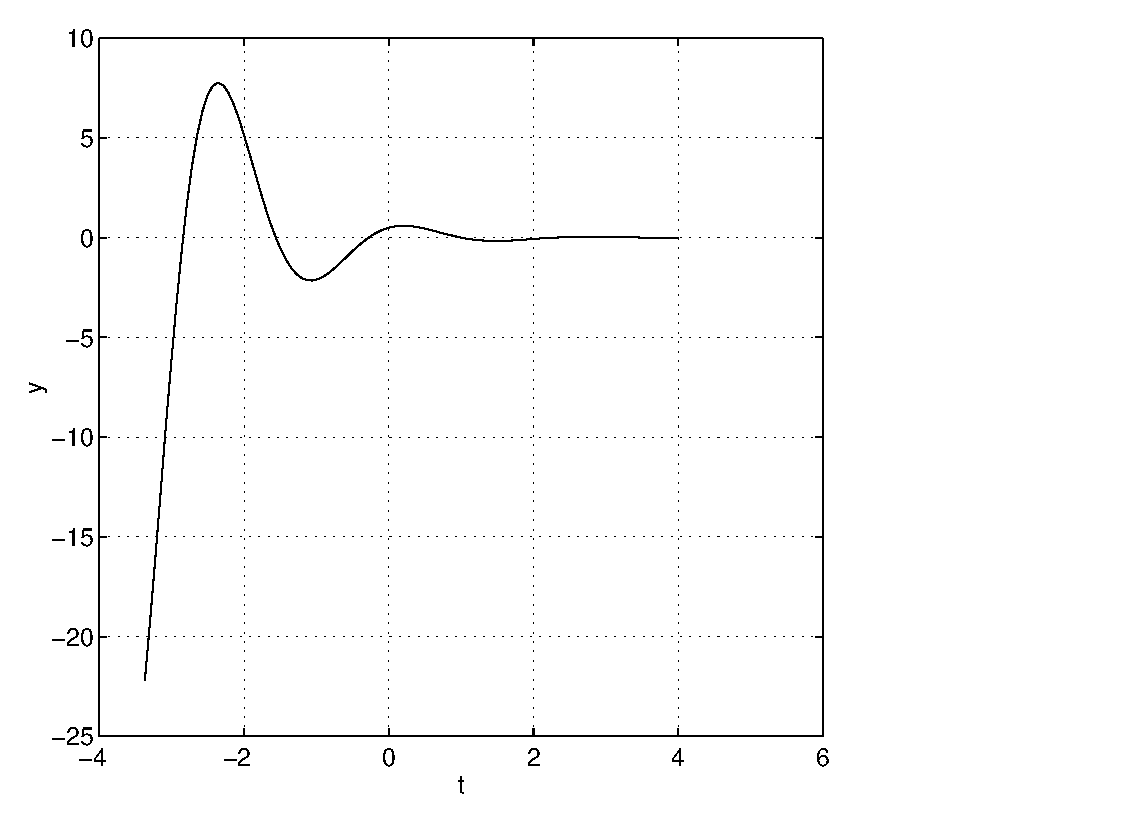
\psfig{file=exfigure/3-5-4.eps,width=3.0in}}
			\exercap{c3.5.4}
\end{figure}

\end{solution}
\end{exercise}

\noindent In Exercises~\ref{c3.5.5a} -- \ref{c3.5.5d}, determine which of
the function pairs $(x_1(t),y_1(t))$ and $(x_2(t),y_2(t))$ are solutions
to the given system of ordinary differential equations.
\begin{exercise} \label{c3.5.5a}
The ODE is:
\begin{eqnarray*}
\dot{x} & = & 2x+y  \\
\dot{y} & = & 3y.
\end{eqnarray*}
The pairs of functions are:
\[
(x_1(t),y_1(t)) = (e^{2t},0)  \AND (x_2(t),y_2(t)) = (e^{3t},e^{3t}).
\]

\begin{solution}
\ans Both function pairs are solutions to the given system.

\soln To determine whether $(x_1(t),y_1(t)) = (e^{2t},0)$ is
a solution to the system, compute the left hand sides of the equations:
\[
\frac{dx_1}{dt}(t) = \frac{d}{dt}(e^{2t}) = 2e^{2t} \AND
\frac{dy_1}{dt}(t) = \frac{d}{dt}(0) = 0.
\]
Then compute the right hand sides of the equations:
\[
2x_1(t) + y_1(t) = 2e^{2t} + 0 = 2e^{2t} \AND
3y_1(t) = 3(0) = 0.
\]
Since the left hand side of each equation equals the right hand side, the
equations are consistent, and the pair of functions is a solution.

\para Similarly, to determine whether $(x_2(t),y_2(t)) = (e^{3t},e^{3t})$
is a solution to the system, compute the left hand sides of the equations:
\[
\frac{dx_2}{dt}(t) = \frac{d}{dt}(e^{3t}) = 3e^{3t} \AND
\frac{dy_2}{dt}(t) = \frac{d}{dt}(e^{3t}) = 3e^{3t}.
\]
Then compute the right hand sides of the equations:
\[
2x_2(t) + y_2(t) = 2e^{3t} + e^{3t} = 3e^{2t} \AND
3y_2(t) = 3e^{3t}.
\]
Since the left hand side of each equation equals the right hand side, the
equations are consistent, and the pair of functions is a solution.


\end{solution}
\end{exercise}
\begin{exercise} \label{c3.5.5b}
The ODE is:
\begin{eqnarray*}
\dot{x} & = & 2x - 3y  \\
\dot{y} & = & x - 2y.
\end{eqnarray*}
The pairs of functions are:
\[
(x_1(t),y_1(t)) = e^t(3,1)  \AND (x_2(t),y_2(t)) = (e^{-t},e^{-t}).
\]

\begin{solution}
\ans Both function pairs are solutions to the given system.

\soln To determine whether $(x_1(t),y_1(t)) = (3e^t, e^t)$ is
a solution to the system, compute the left hand sides of the equations:
\[
\frac{dx_1}{dt}(t) = \frac{d}{dt}(3e^t) = 3e^t \AND
\frac{dy_1}{dt}(t) = \frac{d}{dt}(e^t) = e^t.
\]
Then compute the right hand sides of the equations:
\[
2x_1(t) - 3y_1(t) = 2(3e^t) - 3e^t = 3e^t \AND
x_1(t) - 2y_1(t) = 3e^t - 2e^t = e^t.
\]
Since the left hand side of each equation equals the right hand side, the
equations are consistent, and the pair of functions is a solution.

\para Similarly, to determine whether $(x_2(t),y_2(t)) = (e^{-t},e^{-t})$
is a solution to the system, compute the left hand sides of the equations:
\[
\frac{dx_2}{dt}(t) = \frac{d}{dt}(e^{-t}) = -e^{-t} \AND
\frac{dy_2}{dt}(t) = \frac{d}{dt}(e^{-t}) = -e^{-t}.
\]
Then compute the right hand sides of the equations:
\[
2x_2(t) - 3y_2(t) = 2e^{-t} - 3e^{-t} = -e^{-t} \AND
x_2(t) - 2y_2(t) = e^{-t} - 2e^{-t} = -e^{-t}.
\]
Since the left hand side of each equation equals the right hand side, the
equations are consistent, and the pair of functions is a solution.


\end{solution}
\end{exercise}
\begin{exercise} \label{c3.5.5c}
The ODE is:
\begin{eqnarray*}
\dot{x} & = &  x + y \\
\dot{y} & = & -x + y.
\end{eqnarray*}
The pairs of functions are:
\[
(x_1(t),y_1(t)) =  (3e^t, -2e^t) \AND (x_2(t),y_2(t)) = e^t(\sin t,\cos t).
\]

\begin{solution}
\ans The function pair $(e^t\sin{t},e^t\cos{t})$ is a
solution to the system, while the function pair $(3e^t,-2e^t)$ is not.

\soln To determine whether $(x_1(t),y_1(t)) = (3e^t,-2e^t)$ is
a solution to the system, compute the left hand sides of the equations:
\[
\frac{dx_1}{dt}(t) = \frac{d}{dt}(3e^t) = 3e^t \AND
\frac{dy_1}{dt}(t) = \frac{d}{dt}(-2e^t) = -2e^t.
\]
Then compute the right hand sides of the equations:
\[
x_1 + y_1 = 3e^t - 2e^t = e^t \AND
-x_1 + y_1 = -3e^t - 2e^t = -5e^t.
\]
Since $\frac{dx_1}{dt} \neq x_1 + y_1$ and $\frac{dy_1}{dt} \neq -x_1 + y_1$,
the pair of functions is not a solution.

\para Similarly, to determine whether $(x_2(t),y_2(t)) =
(e^t\sin{t},e^t\cos{t})$ is a solution to the system, compute the left
hand sides of the equations:
\[
\frac{dx_2}{dt}(t) = \frac{d}{dt}(e^t\sin{t}) = 
e^t\sin{t} + e^t\cos{t} \AND
\frac{dy_2}{dt}(t) = \frac{d}{dt}(e^t\cos{t}) =
e^t\cos{t} - e^t\sin{t}.
\]
Then compute the right hand sides of the equations:
\[
x_2(t) + y_2(t) = e^t\sin{t} + e^t\cos{t} \AND
-x_2(t) + y_2(t) = -e^t\sin{t} + e^t\cos{t}.
\]
Since the left hand side of each equation equals the right hand side, the
equations are consistent, and the pair of functions is a solution.


\end{solution}
\end{exercise}
\begin{exercise} \label{c3.5.5d}
The ODE is:
\begin{eqnarray*}
\dot{x} & = & y  \\
\dot{y} & = &  -\frac{1}{t^2}x + \frac{1}{t}y + 1.
\end{eqnarray*}
The pairs of functions are:
\[
(x_1(t),y_1(t)) = (t^2,2t)  \AND (x_2(t),y_2(t)) = (2t^2,4t).
\]

\begin{solution}
\ans The function pair $(t^2,2t)$ is a solution to
the system, while the function pair $(2t^2,4t)$ is not.

\soln To determine whether $(x_1(t),y_1(t)) = (t^2,2t)$ is
a solution to the system, compute the left hand sides of the equations:
\[
\frac{dx_1}{dt}(t) = \frac{d}{dt}(t^2) = 2t \AND
\frac{dy_1}{dt}(t) = \frac{d}{dt}(2t) = 2.
\]
Then compute the right hand sides of the equations:
\[
y_2(t) = 2t \AND
-\frac{1}{t^2}x_1(t) + \frac{1}{t}y_1(t) + 1 =
-\frac{1}{t^2}(t^2) + \frac{1}{t}(2t) + 1 = -1 + 2 + 1 = 2.
\]
Since the left hand side of each equation equals the right hand side, the
equations are consistent, and the pair of functions is a solution.

\para Similarly, to determine whether $(x_2(t),y_2(t)) = (2t^2,4t)$ is a
solution to the system, compute the left hand sides of the equations:
\[
\frac{dx_2}{dt}(t) = \frac{d}{dt}(2t^2) = 4t \AND
\frac{dy_2}{dt}(t) = \frac{d}{dt}(4t) = 4.
\]
Then compute the right hand sides of the equations:
\[
y_2(t) = 4t \AND
-\frac{1}{t^2}x_2(t) + \frac{1}{t}y_2(t) + 1 =
-\frac{1}{t^2}(2t^2) + \frac{1}{t}(4t) + 1 = -2 + 4 + 1 = 3.
\]
Since $\frac{dy_2}{dt} \neq -\frac{1}{t^2}x_2 + \frac{1}{t}y_2 + 1$,
the function pair is not a solution.





\end{solution}
\end{exercise}


\end{document}
